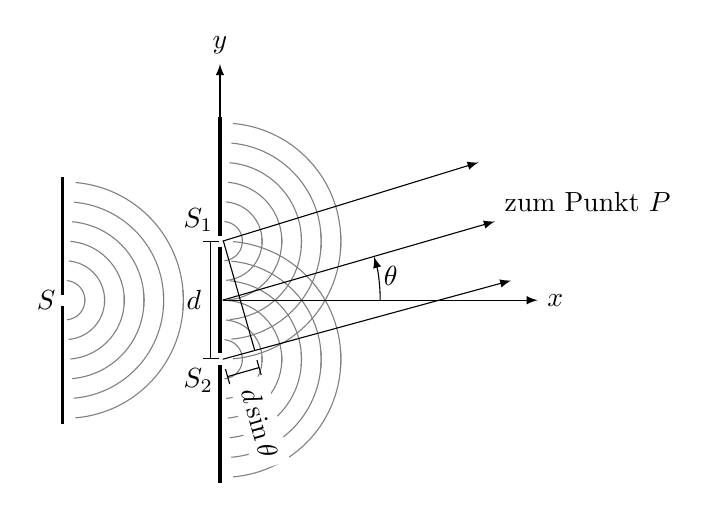
\begin{tikzpicture}[>=latex]
	% first pinhole
	\begin{scope}
		\draw (0,0) node[left] {$S$};
		\foreach \i in {-1,1}
			\draw[xshift=-1,yshift=\i*2,very thick] (0,0) -- (0,\i*1.5);;
		\foreach \r in {1,2,...,6} {
			\draw[scale=\r*.25, rotate=5, color=black!50] (0,-1) .. controls (0.555,-1) and (1,-0.555) .. (1,0);
			\draw[scale=\r*.25, rotate=-5, color=black!50] (0,1) .. controls (0.555,1) and (1,0.555) .. (1,0);
		};
	\end{scope}

	
	% right part
	\begin{scope}[xshift=2cm]
		% pinhole 1
		\begin{scope}[yshift=.75cm]
			\draw (0,0) node[above left] {$S_1$};
			\draw[xshift=-1,yshift=2,very thick] (0,0) -- (0,1.5);
			\draw[xshift=-1,yshift=-2,very thick] (0,0) -- (0,-1.35);
			\foreach \r in {1,2,...,6} {
				\draw[scale=\r*.25, rotate=5, color=black!50] (0,-1) .. controls (0.555,-1) and (1,-0.555) .. (1,0);
				\draw[scale=\r*.25, rotate=-5, color=black!50] (0,1) .. controls (0.555,1) and (1,0.555) .. (1,0);
			};
		\end{scope}

		% pinhole 2
		\begin{scope}[yshift=-.75cm]
			\draw (0,0) node[below left] {$S_2$};
			\draw[xshift=-1,yshift=-2,very thick] (0,0) -- (0,-1.5);
			\foreach \r in {1,2,...,6} {
				\draw[scale=\r*.25, rotate=5, color=black!50] (0,-1) .. controls (0.555,-1) and (1,-0.555) .. (1,0);
				\draw[scale=\r*.25, rotate=-5, color=black!50] (0,1) .. controls (0.555,1) and (1,0.555) .. (1,0);
			};
		\end{scope}
	
		% distance
		\begin{scope}[xshift=-.15cm]
			\draw[|-|] (0,-.75) -- (0,.75) node[pos=.5, left] {$d$};
		\end{scope}
		
		% x-scale
		\draw[thin,->] (0,0) -- (4,0) node[right] {$x$};
		
		% y-scale
		\draw[thin,->,xshift=-1] (0,2) -- (0,3) node[above] {$y$};
		
		\foreach \i in {0,1,2} {
			\draw[->,yshift=(\i-1)*-.75cm] (0,0) -- (3.25+0.2756*\i*.75,1);
		};
		\draw[rotate=16,xshift=.215cm,yshift=-.725cm] (0,0) -- (0,1.45);
		\draw (3.457,1) node[above right] {zum Punkt $P$};
		
		\draw[->] (2,0) arc (0:16:2) node[below right] {$\theta$};
		
		\draw[|-|,rotate=16,yshift=-.95cm] (-0.215,0) -- (0.215,0) node[rotate=-74,pos=.55,right,xshift=.1cm,fill=white] {$d\sin\theta$};
	\end{scope}
\end{tikzpicture}